\documentclass{article}

\usepackage{hyperref}
%\hypersetup{colorlinks, %
%	citecolor=black,%
%	filecolor=black,%
%	linkcolor=black,%
%	urlcolor=black,%
%	pdftex}	
\usepackage{graphicx}
\usepackage{tikz}
\usepackage{amssymb,amsmath}
\usepackage{float}
\newcommand{\email}[1]{\texttt{#1}}
\newcommand{\gmat}{GMAT}
\newcommand{\vim}{\href{http://www.vim.org} {www.vim.org} }

\title{\gmat{} Maths Grinds}
\author{Conor Gilmer $<$\href{mailto:conor.gilmer@gmail.com}{conor.gilmer@gmail.com}$>$}


\begin{document}
\pagestyle{headings}
\maketitle

\tableofcontents


\newpage
\section{The Prologue}
I\footnote{\email{ \href{mailto:conor.gilmer@gmail.com.com}{conor.gilmer@gmail.com} }} am just going to outline the rules and formulae which are needed for the GMAT Mathematics test.

\section{Topics}

The topics covered

\begin{itemize}
\item Geometry - Area and Perimeter of shapes, and Surface Area and Volume.
\item Algebra - solve equations, factoring, inequalities
\item Arithmetic - working out the results
\item Problem Solving - word problems
\end{itemize}


\newpage
\section{Prerequistes and Definitions}
\subsection{Numbers}
\begin{itemize}
\item {\textbf{Natural Number} - a number which occurs in nature, an integer, a positive whole number e.g. 1,2,3,4,511 etc.}
\item {\textbf{Real Number} - any number which can be plotted on a line \\ e.g $3, 2/3, -0.2, \sqrt{3}$}
\item \textbf{Imaginary Number} - a number which can not be calculated e.g. $\sqrt{-5}$
\item \textbf{Rational Number} - a number which can be written as a fraction e.g. $4 (4/1) , 2/3$
\item \textbf{Irrational Number} - a number which can not be written as a fraction e.g $\sqrt{2}, \pi, 0.271271271271...$
\end{itemize}

\subsection{Multiplying Signed Numbers}

$+a * +b = +ab$

$+a * -b = -ab$

$-a * +b = -ab$

$-a * -b = +ab$

\subsection{Exponents or Indices}
Exponents are the 'power' of a number, so the number of times a number is multiplied by itself e.g.

$x^{3} = x * x * x$

A Negative exponent equates to 1 divided by that number multiplied by itself e.g.

$x^{-4} = \frac{1}{(x * x * x * x)}$

$ 10^{-3}  = \frac{1}{1000} = 0.001 $


Multiplying numbers with exponents you add the exponents 

$a^{2} * a^{3} = a^{2+3} = a^{5}$

Dividing numbers with exponents you subtract the exponents of the divisor number from the number 

$a^{3} / a^{2} = a^{3-2} = a^{1} = a$

$a^{2} / a^{3} = a^{2-3} = a^{-1} = 1/a$

$ a^{x} * b^{x} = ab^{x}$

$ (a/b)^{x} = a^{x} / b^{x} $

$ (a^{x})^{y} =  (a^{y})^{x}  = a^{xy}$


Zero to the power of a number is zero

$ 0^{x} = 0 \quad \textrm{e.g.} \quad  0^{1} = 0$

A number to the power of zero is one

$ x^{0} = 1 \quad \textrm{e.g.} \quad  x^{0 =1}$

Multiplying across by a number 
$a^{2} + a = a (a + 1) $

$a^{3} + a^{2} + 2a = a (a^{2} + a  + 2 )$

\subsection{Ratio}
The Ratio of A to B is written as $ A/B \ or \ A : B$

\subsection{Percentage}
To get a percentage of a fraction your multiply by 100 so $ ( 3/4 ) * 100 = 75\%$

\subsection{Absolute Value}
The \textit{Absolute Value} of a number is the square root of a number squared, so it is always a positive value. 

The \textit{absolute value} of a number 'a' is written as $|a|$.

$ |a| = \sqrt{a^{2}}$ 

The absolute value of a number is often used to get its value, ignoring the sign e.g. the length of a line, where the sign is the direction,



\newpage
\section{Geometry}

\begin{itemize}
\item Lines
\item Four-sided figures
\item Triangles
\item Pythagoras
\item Circles
\item Volume and Surface Area
\item Polygons
\end{itemize}

\subsection{Lines}
A Line is said to be 180 $\circ$, so if you know the angle one makes intersecting a line you know the other side
\subsection{Intersecting Lines}
The opposite angles in intersecting lines are equal.
\subsection{Line intersecting Parallel Lines}
Parallel lines the angles are preserved, i.e. the angles made by the intersecting lines are the same

\newpage
\subsection{Four-sided figures}
\begin{enumerate}
\item Rectangles
\item Squares
\item Parallelograms
\item Other foursided figures
\end{enumerate}
\subsubsection{Area of a Rectangle}
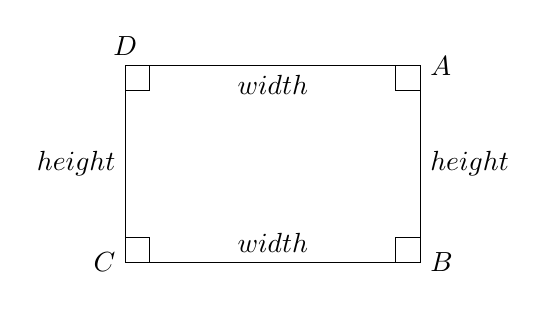
\begin{tikzpicture}[scale=1.25]%,cap=round,>=latex]

\coordinate [label=left:$C$] (A) at (-1.5cm,-1.0cm);
\coordinate [label=right:$B$] (B) at (1.5cm,-1.0cm);
\coordinate [label=right:$A$] (C) at (1.5cm,1.0cm);
\coordinate [label=above:$D$] (D) at (-1.5cm,1.0cm);

\draw (A) -- node[above] {$width$} (B) -- node[right] {$height$} (C) -- node[below] {$width$} (D) -- node[left] {$height$} (A);

\draw (1.25cm,-1.0cm) rectangle (1.5cm,-0.75cm);
\draw (-1.5cm,-1.0cm) rectangle (-1.25cm,-0.75cm);

\draw (-1.5cm,1.0cm) rectangle (-1.25cm,0.75cm);
\draw (1.5cm,1.0cm) rectangle (1.25cm,0.75cm);

\end{tikzpicture}

Area of a rectangle is the length of the sides multiplied together.
\begin{equation}
Area_{\;rectangle} = width * height
\end{equation}
\subsubsection{Perimeter of a Rectangle}
Is the sum of the 4 sides
\begin{equation}
\begin{split}
Perimeter_{\;Rectangle} =  2\;width\;+\;2\;height
\\Perimeter_{\;rectangle} = 2 (width\;+\;height)
\end{split}
\end{equation}

\subsubsection{Square}
Well a square is just a rectangle where all the sides are the same size, so all the rules apply but just are simpler.

\subsubsection{Parallelogram}
A parallelogram is a four-sided figure where the the sides are parallel, opposite sides are equal and opposite angles are equal.
The only property which changes is the area

$Area_{Parallelogram} = base * perpendicular-height$

$Sum\;of\;the\;Angles\;in\;a\;Parallelogram  = 360^{\circ}$


\newpage
\subsection{Triangles}
\begin{enumerate}
\item Perimeter of a Triangle equals sum of 3 sides
\item Area of a Triangle equals half the base by perpendicular height
\item The sum of the angles of a triangle equal $180^{\circ}$
\item Equilateral Triangle - all the angles are $60^{\circ}$, and all sides are the same length
\item Isosceles Triangle - 2 angles are the same and 2 sides are the same length
\end{enumerate}
\subsubsection{Perimeter of a Triangle}
Perimeter of a triangle is the sum of the 3 sides so
Perimeter = Side A + Side B + Side C
\subsubsection{Area of a Triangle}
\begin{equation}
Area_{Triangle} = base * Perpindicular Height / 2
\end{equation}
\subsubsection{Angles in a Triangle}
The angles in a triangle equal $180^{\circ}$
So if you have two angles you always can deduct the third.
\newpage
\subsection{Pythagoras Theorem}
The most important theorem In a Right angle triangle(one angle = $90^{\circ}$), the square on the hypoteneuse (longest side) is equal to the sum of the squares on the other two sides

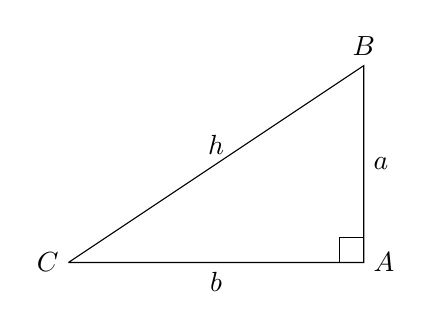
\begin{tikzpicture}[scale=1.25]%,cap=round,>=latex]

\coordinate [label=left:$C$] (A) at (-1.5cm,-1.cm);
\coordinate [label=right:$A$] (C) at (1.5cm,-1.0cm);
\coordinate [label=above:$B$] (B) at (1.5cm,1.0cm);
\draw (A) -- node[above] {$h$} (B) -- node[right] {$a$} (C) -- node[below] {$b$} (A);

\draw (1.25cm,-1.0cm) rectangle (1.5cm,-0.75cm);

\end{tikzpicture}

\begin{equation}
h^2 = a^2 + b^2
\end{equation}
so $h= \sqrt{a^2 + b^2}$
\subsubsection{Also works for the Circle on the Hypoteneuse}
As a result the circle on the hypoteneuse is equal to the sum of the circle of the other two sides.

\begin{equation}
\pi (h/2)^2 = \pi (a/2)^2 + \pi(b/2)^2
\end{equation}

You will find that often the numbers used in examples are triangles with sides 5, 4 and 3, 10, 8 and 6 or 50, 40 and 30 which all neatly square etc.

\newpage
\subsection{Circles}
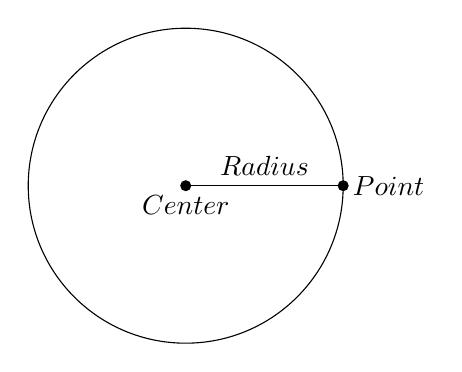
\begin{tikzpicture}
\coordinate [label=below:$Center$] (A) at (2,2);
\coordinate [label=right:$Point$] (B) at (4, 2);
\draw (2,2) circle (2cm);
\draw (A) -- node[above] {$Radius$} (B);
\foreach \dot in {A, B} {
  \fill (\dot) circle(2pt);
  %\node[above] at (\dot) {\dot};
}
\end{tikzpicture}
\subsubsection{Area of a Circle}
\begin{equation}
Area_{ Circle} = \pi r^ 2
\end{equation}
\subsubsection{Circumference of a Circle}
\begin{equation}
Circumference_{ Circle} = 2 \pi r
\end{equation}
\subsection{Sectors of a Circle}
A sector of a Circle of is a portion of a circle like a slice of pizza or tart with two straight lines from the centre of the circle out to the edge. The Angle is the angle between the two straight lines from the centre of the circle.
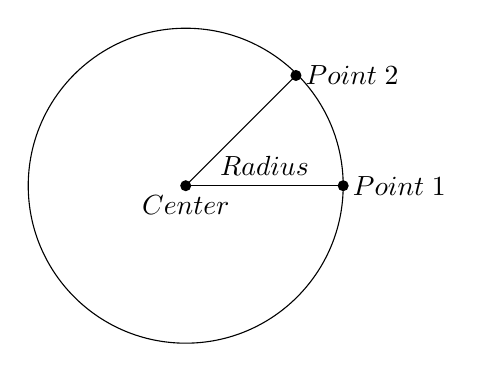
\begin{tikzpicture}
\coordinate [label=below:$Center$] (A) at (2,2);
\coordinate [label=right:$Point\;1$] (B) at (4, 2);
\coordinate [label=right:$Point\;2$] (C) at (3.4, 3.4);
\draw (2,2) circle (2cm);
\draw (A) -- node[above] {$Radius$} (B);
\draw (A) -- (C);
\foreach \dot in {A, B, C} {
  \fill (\dot) circle(2pt);
  %\node[above] at (\dot) {\dot};
}
\end{tikzpicture}
\subsubsection{Area of a Sector of a Circle}
\begin{equation}
Area_{ Sector\;of\;a\;Circle} = ( \frac{Angle }{ 360 }) \pi r^ 2
\end{equation}


\subsubsection{Circumference of a Sector of a Circle}
\begin{equation}
Circumference_{ Sector\;of\;a\;Circle} = ( \frac{Angle }{ 360} ) 2 \pi r
\end{equation}

\subsection{Polygons}
\subsubsection{Area of a Polygon}
To get a polygons area, you \textit{break it up into triangles} or triangles and rectangles, you may need to use pythagoras.
\subsubsection{Perimeter of a Polygon}
The sum of the lengths of its sides
\subsubsection{Sum of angles of a polygon}
Sum of the triangles which meet the points of the polygon - i.e. multiples of 180
Or triangle is 180, rectangle 360, adding another side will always be adding another triangle so
pentagon is 540, hexagon is 720 and heptagon is 900 and octagon 1060 and so on...


\newpage
\subsection{Volume and Surface Area}
\subsubsection{Rectangular Box}
\begin{itemize}
\item Volume of a Rectangular Box - Length by Breath by Height
\item Surface Area, is six rectangle, two breath by depth plus two breath by height plus two height by depth
\end{itemize}

\begin{equation}
Volume = width * height * depth
\end{equation}

\begin{equation}
Surface\;Area = 2(width * height) + 2(width * depth) + 2(height * depth)
\end{equation}

\subsubsection{Cylinder}
\begin{itemize}
\item Volume of a Cylinder is area of the base by the height
\item Surface area is 2 circles and a rectangle (from the rolled out tube of the cylinder) height by circumference of the circle
\end{itemize}

\begin{equation}
Volume_{ Cylinder} = h \pi r^ 2
\end{equation}


\begin{equation}
Surface\;Area_{ Cylinder} = 2 \pi r h + 2(\pi r^ 2 )
\end{equation}

\subsubsection{Sphere}
A sphere is an object like a ball, where the distance from the centre of the object to the edge is the radius. For GMAT your supposed to know what a sphere is but not required to know how to get its volume or surface area.
However if you're curious 
\begin{equation}
Volume_{Sphere} = \frac{4}{3} \pi r^{3}
\end{equation}
\begin{equation}
Surface\;Area_{Sphere} = 4 \pi r^{2}
\end{equation}

\newpage
\subsection{Coordinate Geometry}
\subsubsection{Plotting a line}
To plot a line on the x-y axis if you have two points with co-ordinates $a = (1,1)$ and $y = (2,3)$ you plot the two points on the axis and draw a line between them.

%\begin{tikzpicture}
%    \draw [thin, gray, ->] (0,-1) -- (0,3)      % draw y-axis line
%        node [above, black] {$y$};              % add label for y-axis
%    \draw [thin, gray, ->] (-1,0) -- (3,0)      % draw x-axis line
%        node [right, black] {$x$};              % add label for x-axis
%    \draw [draw=red,ultra thick] (1,1) -- (3,2);% draw the graph
%    \node [left] at (1,1) {$(1,1)$};                % label y-intercept
%   \node [above] at (3,2) {$(3,2)$};               % label x-intercept
%\end{tikzpicture}


\begin{tikzpicture}
\draw [thick,->] (0,0) -- (4.5,0) node[anchor=north west] {x axis};
\draw [thick,->] (0,0) -- (0,4.5) node[anchor=south east] {y axis};
\foreach \x in {0,1,2,3,4}
    \draw (\x cm,1pt) -- (\x cm,-1pt) node[anchor=north] {$\x$};
\foreach \y in {0,1,2,3,4}
    \draw (1pt,\y cm) -- (-1pt,\y cm) node[anchor=east] {$\y$};
    
\draw [draw=red,ultra thick] (1,1) -- (3,2);% draw the graph

    \node [left] at (1,1) {$(1,1)$};                % label y-intercept
    \node [above] at (3,2) {$(3,2)$};               % label x-intercept
\end{tikzpicture}


\subsubsection{Length of a line between two points on the plane}
Finding the length of a line on a plane, involves plotting it on an $x y $ axis. The length of a line can be worked out by using Pythagoras. So the length of a line from a (1,-3) and b (-1, 2) is $ \sqrt{2^{2} + (-5)^{2}}$.
 
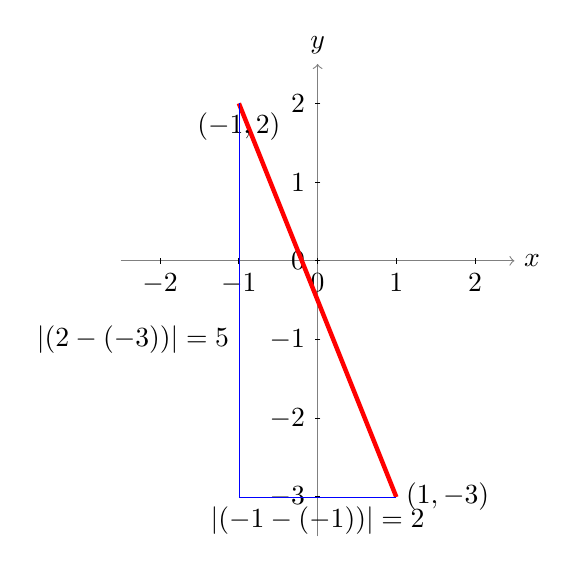
\begin{tikzpicture}
    \draw [thin, gray, ->] (0,-3.5) -- (0,2.5)      % draw y-axis line
        node [above, black] {$y$};              % add label for y-axis

    \draw [thin, gray, ->] (-2.5,0) -- (2.5,0)      % draw x-axis line
        node [right, black] {$x$};              % add label for x-axis

\foreach \x in {-2,-1, 0,1,2}
    \draw (\x cm,1pt) -- (\x cm,-1pt) node[anchor=north] {$\x$};
\foreach \y in {-3,-2,-1,0,1,2}
    \draw (1pt,\y cm) -- (-1pt,\y cm) node[anchor=east] {$\y$};
    

    \draw [draw=red,ultra thick] (1,-3) -- (-1,2);% draw the graph

    \node [right] at (1,-3) {$(1,-3)$};                % label y-intercept
    \node [below] at (-1,2) {$(-1,2)$};                % label x-intercept
    
    \draw [draw=blue,ultra thin] (-1,2) -- (-1,-3);% draw the graph
    \node [left] at (-1,-1) {$|(2 -(-3))| = 5$};
    \draw [draw=blue,ultra thin] (-1,-3) -- (1,-3);% draw the graph
    \node [below] at (0,-3) {$|(-1 -(-1))| = 2$}; 
    
\end{tikzpicture} 
 
\newpage
\subsubsection{Slope of a Line}
There are two ways which get you the slope of a line one is with the co-ordinates the other with an equation which you resolve to look like y = mx + b where m is the slope of the line

\textbf{Using the Equation}

\begin{equation}
y = mx + B
\end{equation}

\textbf{Using Co-ordinates}

With co-ordinates ($x_1$, $y_1$) and ($x_2$, $y_2$) 
\begin{equation}
m = \frac{ (y_2 - y_1) }{ (x_2 - y_1) }
\end{equation}


\textit{Caveat if the slope of a line m is positive the line goes upwards from left to right, and if the slope is negative then it goes downwards.}

\subsubsection{Functions}
A \textit{function} relates an input to an output, often the output is expressed as an expression/equation.
e.g. $f(x) = x^2 - 6 $ is a function which you can plot on an x-y axes, where each point will $(x,f(x))$ . 


\begin{table}
\begin{tabular}{l|l|l}
$x$ & $ x^{2} - 6 = f(x)$& $(x,\;f(x))$  \\
\hline
-2 & $-2^{2} -6 = -2$ & $(-2,\;-2)$  \\
-1 & $-1^{2} -6 = -5$ & $(-1,\;-6)$  \\
0 & $0^{2} -6 = -6$ & $(0,\;-6)$  \\
1 & $1^{2} -6 = -6$ & $(1,\;-6)$  \\
2 & $2^{2} -6 = -2$ & $(2,\;-2)$  \\
3 & $3^{2} -6 = 3$ & $(3,\;-3)$  \\
4 & $4^{2} -6 = 10$ & $(4,\;10)$ \\

\end{tabular}
\caption{\label{•}}
\end{table}

\newpage
\section{Algebra}
\subsection{Solve an Equation one Variable}
In this case you just manipulate the equation so as the variable is on one side on its own and what it equals is on the other.

$2x - 9 = 1$

$2x = 1 + 9 $

$2x = 10 $

$x = 10 /2  \;so \; x = 5$

\subsubsection{Two Equations with Two Variables}
Solved by getting what one variable is as an expression of the other then plug it in

$2x -3y = 1 $  
       
$x + 2y = 11 $	     

$x = 11 -2y$

$22-4y -3y = 1$

$22 - 7y = 1$

$-7y = 1-22$

$-7y = -21$

$7y = 21$

$y =21/7   \;so \;  y = 3$

So since you now know $y$ you can work out $x$

$x + 3 (3) = 11$
$x = 11 -9 = 2$

\newpage
\subsection{Quadratic Equations}
A \textit{Quadratic Equation} is an equation of the form $ax^{2} + bx + c = 0$ (Quadratic just means the function contains a squared variable).

\begin{itemize}
\item Factoring
\item Using Quadratic Formula
\item Completing the Square
\end{itemize}

\subsubsection{Factoring}
Solve an equation by simplifying and factoring, factoring is finding out what is multiplied that gives you the quadratic equation

Often the key is recognising patterns and knowing how combinations of factors multiply you can work out what the factors are 

$a^{2} + 2ab + b^{2} = (a + b) (a + b)  = (a + b)^{2}$

$a^{2} - 2ab + b^{2} = (a - b) (a - b)  = (a - b)^{2}$

$a^{2} - b^{2} = (a + b) (a - b)$


Multiplying across

$2a^{3} -4a^{2}b + 2ab^{2} = 2a ( a^{2} - 2ab + b^{2} ) = 2a (a-b)^{2}$

To solve an equation by factoring you move all the elements to one side so as it equals to 0,
then you try and reduced the equation to what it will.
Ultimately you are find what are the possible values for the variable.


\subsubsection{Quadratic Formula}
Solve the equation by using the \textit{Quadratic Formula}  
So for $ax^{2} + bx + c = 0$
\begin{equation}
x = \frac{-b \pm \sqrt{b^{2}-4ac}}{2a}
\end{equation}

\textbf{For Example} 
Solve $5x^{2} + 6x + 1 = 0\\$
$a = 5\;; b = 6\;; c = 1\;;$

Put into formula

$\frac{-6 \pm \sqrt{6^{2} - 4 (5) (1)}}{2 (5)}\\
\frac{-6 \pm \sqrt{36-20}}{10}\\
\frac{-6 \pm \sqrt{16}}{10} \\
\frac{-6 \pm 4}{10} \\
x = -\frac{1}{5}\;\; or -1$


\subsubsection{Completing the Square}
$2 x^{2} - 12 x - 9 = 0\\
2 x^{2} - 12 x = 9 \\
x^{2} -6 x = \frac{9}{2}$

Make the left hand side look like a factor-able function in this case by adding $9$ to both sides.

$x^{2} -6 x  + 9 = \frac{9}{2} + 9\\
(x-3) (x -3) = \frac{9}{2} + 9\\ 
(x-3)^{2} = \frac{9}{2} + \frac{18}{2} = \frac{27}{2}\\
x-3 = \pm \sqrt{\frac{27}{2}} \\
x = \pm \sqrt{\frac{27}{2}} + 3 \\
x = 3 \pm \sqrt{\frac{9 . 3}{2}} \\
x = 3 \pm 3\sqrt{\frac{3}{2}} = 3 \pm 3\sqrt{\frac{6}{4}} \\ 
x = 3 \pm 3\frac{\sqrt{6}}{\sqrt{4}} \\ 
x = 3 \pm 3\frac{\sqrt{6}}{2} $ So you have two solutions.

\subsection{Inequalities}
\subsubsection{Symbols}
\begin{tabular}{l|l|l}
$Symbol$ & $Meaning$ & $Usage$  \\
\hline
$<$ & $Less\;than$ & $ 5 < 10$  \\
$>$ & $Greater\;than$ & $ 51 > 49$  \\
$\leq$ & $Less\;than\;or\;equal\;to$ & $ p \leq 10$  \\
$\geq$ & $Greater\;than\;or\;equal\;to$ & $ Age \geq 18$  \\
\hline
\end{tabular}

\newpage
\section{Arithmetic}
\subsection{Statistics}

\subsubsection{Average/Mean}
In Statistics the \textit{Mean} is the average of the sequence numbers (sometimes referred to as the \textit{arithmetic mean}.

$
Mean = \frac{A + B + C + D + ...}{Number\; of\; Numbers}
$

\subsubsection{Median}
Roughly is the middle number of a sequence, it is either the middle number or the average of the 2 middle numbers.

\subsubsection{Range}
The \textit{range} is the span from the lowest number to the highest number.

\subsubsection{Mode}
The \textit{Mode} of a list of numbers is the most frequently occurring number or numbers.

\subsubsection{Standard Deviation} 


$\\
List =  0, 7, 8 , 10, 10 
\\
Number\; of\; numbers\; in\; the\; squence\; =\; 5
\\
Mean = \frac{0 + 7 + 8 + 10 + 10}{5} =  7
$

\begin{table}[H]

\begin{tabular}{l|ll}
$x$ & $(x - 7)$ & $(x -7)^{2}$  \\
\hline
0 & -7 & 49  \\
7 & 0 &  0 \\
8 & 1 & 1  \\
10 & 3 & 9  \\
10 & 3 & 9  \\
\hline

Total & is & 68  \\
\end{tabular}

\caption{\label{tab:widgets}Calculating the Standard Deviation.}
\end{table}

$Standard\;Deviation \;\; \sigma = \sqrt{\frac{68}{5}}$

\newpage
\subsubsection{Factorials}
A factorial of a number is the product of all the postive integers less than or equal to that number.
Notation $n!$

$\\ 2! = 2 * 1 = 2 \\$
$ 5! = 5 * 4 * 3 * 2 * 1 = 120\\ $
$ 10! = 10 * 9 * 8 * 7 * 6 * 5 * 4 * 3 * 2 * 1 = 3,628,800 $

Caveat $0! = 1 $

\subsubsection{Simplifying Factorials}
$\left(\frac{10!}{5!2!}\right) = \left(\frac{10 * 9 * 8 * 7 * 6 * 5 * 4 * 3 * 2 * 1}{(5 * 4 * 3 * 2 * 1)(2 * 1)}\right)\\
\left(\frac{10 * 9 * 8 * 7 * 6 * 5 * 4 * 3 * 2 * 1}{(5 * 4 * 3 * 2 * 1)(2 * 1)}\right) = \frac{10 * 9 * 8 * 7 * 6 }{2} = 15120
$

\newpage
\subsection{Probability}
Probability of an event is the number of results over the total number of possible results.
\begin{equation}
P(E) = \frac{Number\;of\;outcomes}{Total\;number\;of\;possible}
\end{equation}
\textbf{e.g}
If you throw a dice twice what are the chances (probability) of 1 side being shown.

$P(E) = \frac{2}{6} = \frac{1}{3}$

This often described as a $1$ in $3$ chance of occurring.

\subsubsection{Probability Arithmetic}
Rule of thumb in combining probability is if you have two events, and you want to know the probability of 
\begin{itemize}
\item Probability of Event A \textbf{AND} Event B =  $P(A) * P(B)$
\item Probability of Event A \textbf{OR} Event B =  $P(A) + P(B)$
\item Probability of an Event E \textbf{NOT} occurring $P(NOT E) = P(\overline{E}) = 1 - P(E)$
\end{itemize}

\textbf{e.g}
If you throw two dice (Dice A and Dice B) at the same time, what are the chances (probability) of the number 6 been shown on (1) both the dice A AND dice B, (2) Probability or either dice A OR dice B being the number 6 and (3) chances of the number 6 NOT landing on both dice A AND dice B.

(1)

$\\P(A\;AND\;B) = P(A) * P(B) \\
P(A\;AND\;B) = \frac{1}{6} * \frac{1}{6} \\
P(A\;AND\;B) = \frac{1 * 1}{6 * 6} = \frac{1}{36}
$

(2)

$\\P(A\;OR\;B) = P(A) + P(B) \\
P(A\;OR\;B) = \frac{1}{6} + \frac{1}{6} \\
P(A\;OR\;B) = \frac{1 + 1}{6} = \frac{2}{6} = \frac{1}{3}
$

(3)

$\\NOT\;(P(A\;AND\;B)) = 1 - (P(A) * P(B)) \\
NOT \;P(A\;AND\;B) = 1 - (\frac{1}{6} * \frac{1}{6}) \\
NOT \; P(A\;AND\;B) = 1 -(\frac{1 * 1}{6 * 6}) = 1 - (\frac{1}{36}) = \frac{36-35}{36} = \frac{35}{36}
$

\newpage
\subsection{Sets}
A Set is a collection of objects, in mathematics it is generally a collection of numbers but could be other objects.
\begin{itemize}
\item \textbf{Union} A Union B is all the contents of sets A and B - $A \cup B$
\item \textbf{Intersection} A intersection B is the contents which are common to A and B - $A \cap B$ 
\end{itemize}
\subsubsection{Venn Diagram}
Sets can be represented diagramatically using Venn Diagrams.

\textbf{A Union B}
\begin{center}
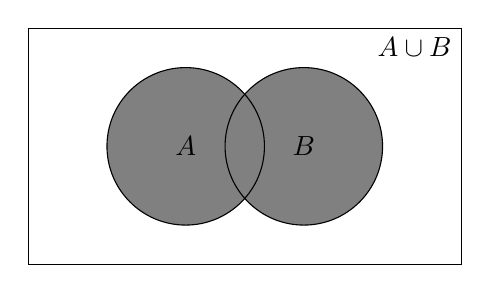
\begin{tikzpicture}
\draw (-2,-1.5) rectangle (3.5,1.5) node[below left]{$A \cup B$};
\fill[gray] (0,0) circle (1cm);
\fill[gray] (1.5,0) circle (1cm);
\draw (0,0) circle (1cm) node {$A$};
\draw (1.5,0) circle (1cm) node {$B$};
\end{tikzpicture}
\end{center}

\textbf{A Intersection B}
\begin{center}
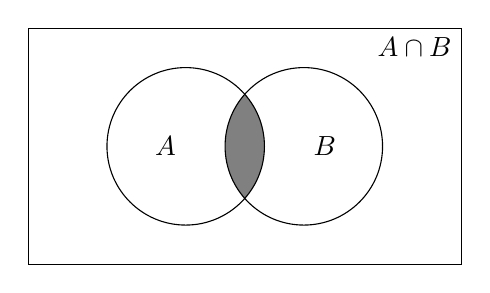
\begin{tikzpicture}
\draw (-2,-1.5) rectangle (3.5,1.5) node[below left]{$A \cap B$};
\begin{scope} % start of clip scope
\clip (0,0) circle (1cm);
\fill[gray] (1.5,0) circle (1cm);
\end{scope} % end of clip scope
\draw (0,0) circle (1cm) node[left] {$A$};
\draw (1.5,0) circle (1cm) node[right] {$B$};
\end{tikzpicture}
\end{center}


\textbf{A Intersection B NOT C}
\def \setA{ (0,0) circle (1cm) }
\def \setB{ (1.5,0) circle (1cm) }
\def \setC{ (60:1.5) circle (1cm) }
\def \setU{ (-2, -1.5) rectangle (3.5, 2.75) }
\begin{center}
\begin{tikzpicture}
\draw \setU node[below left]{$A \cap B \cap \overline{\rm C}$};
\begin{scope}
\clip \setA;
\fill[gray] \setB;
\end{scope}
\begin{scope}
\clip \setA;
\clip \setB;
\fill[white] \setC;
\end{scope}
\draw \setA node[left] {$A$};
\draw \setB node[right] {$B$};
\draw \setC node {$C$};
\end{tikzpicture}
\end{center}


\newpage
\section{Colophon}

Wouldn't have been possible without Mr Euclid and Mr Pythagoras (and maybe Mr Archimedes).

This document was written created using \LaTeX{}. 

Initially it was word-processed using text editor \href{http://www.vim.org}{www.vim.org} and then rendered into pdf using pdflatex. Latterly \href{http://www.xm1math.net/texmaker}{TexMaker} (The Universal LaTeX editor) was used.

The amendments from the original version were made using Version 2.4 of MiKTeX(\href{http://www.miktex.org}{www.miktex.org})
However since using the macbook a lot of late I use \TeX{} Live ( \href{https://www.tug.org/texlive/}{www.tug.org/texlive/}).


%It was tested using the Adobe $^{\textregistered}$ Reader 7.0 (Version 7.0.3).


K.A. Stroud\cite{stroudengmath} was my go to book in college for mathematics as well as the \textit{Red Notes}\cite{rednotes}, and as many in the irish education system Holland and Madden books taught me maths\cite{hollandmadden} in school.

There are many helpful websites online one I found was \textit{Maths is Fun}\cite{mathsisfun}.


\bibliographystyle{plain}
\bibliography{ref}




\copyright 2015 Conor Gilmer $<$\href{mailto:conor.gilmer@gmail.com}{conor.gilmer@gmail.com}$>$ all rights reserved.

\end{document}

